\section{Scenario's}
De scenario view is een representatie van de blangrijkste usecases en interactie tussen de abstracte componenten van het systeem \parencite{4+1ViewModelPaper}.
De user cases zijn opgesteld doormiddel van de geprioriteerde lijst van requirements van het onderzoek \parencite{DanteOnderzoek}.
Om de verschillende usecases en interactie met andere actoren in het systeem in beeld te krijgen wordt er gebruik gemaakt van een usecase diagram \parencite{UseCaseDiagram}.

\whitespace
Alle verschillende user stories zijn vertegenwoordigt in het usecase diagram zie figuur \ref{fig:UseCaseDiagram}.
Het Content plaatsen vertegenwoordigt de stories (KB-FR 1,4,5,8,9,10, SW-FR14 en SW-FR15).
Vormgeven van de content wordt gerpresenteerd door de user stories KB-FR3, KB-FR7 en SW-13.
De Content Bekijken van vertegenwoordigt door KB-FR12 en het inloggen door KB-FR6.

\whitespace[2]
\begin{graphic}
	\captionsetup{type=figure}
	\caption{Use case diagram}
	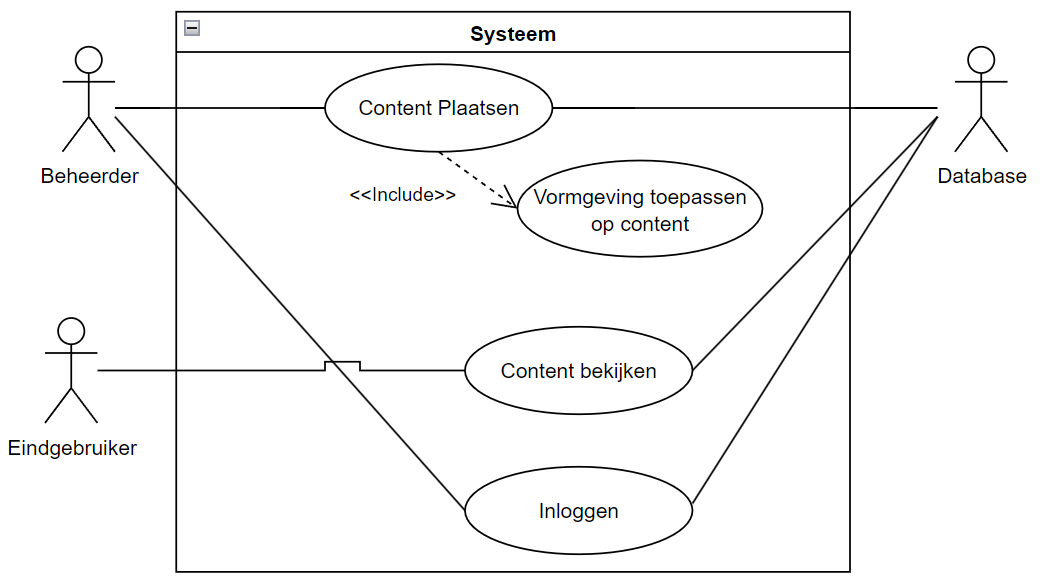
\includegraphics[scale=0.8]{UseCaseDiagram.png}
	\label{fig:UseCaseDiagram}
\end{graphic}

